\chapter{Main Body}
\label{cha:Main Body}


\section{''Pflichtenheft''}
\label{sec:Pflichtenheft}

\subsubsection{Cost}
I've already bought two \acs{devboard}s one of them stays at \acs{tbz} and the other is at home. One of these boards was paid by Mr. Malacarne. Further expenses from the \acs{pcb} will be paid by me and shouldn't exceed about 50 CHF, as the \acs{hw} isn't that complicated.

\subsubsection{Time}
The most time of the project I will work at home because it's a rather big project to execute in one semester. I will also have much time in the fall holidays to work on it. The project will approximately take 100h to complete. Also the more detailed timeplan is in chapter: [\ref{sec:GANTT Chart}]

\subsubsection{Tools}
To realize this project I will mainly use, the \acs{sw} STM32CubeIDE with \acs{hal} and Altium Designer. The documentation is written in LaTeX in VSCode. And I'm planning to order the \acs{pcb} on JLCPCB and I will populate and reflow the PCB at ETHZ, where I'm also allowed to use the measurement equipment for the HW tests.

\subsubsection{Technical Details}
\begin{table}[H]
    \centering
    \label{tab:Technical Details}
\begin{tabular}{||c || c | c | c | c  || c ||} 
 \hline
 value &  min. & typ. & max. & unit & description \\ [0.5ex] 
 \hline\hline
  supply voltage & & 5 & & V & over USB \\ 
 \hline
 curent to measure & 0 & & 1 & A & \\ 
 \hline
 voltage to measure & 0 & & 10 & V & \\ 
 \hline
\end{tabular}
    \caption{Technical Details}
\end{table}

\newpage


\section{Extension PCB}
\label{sec:Extension PCB}



\subsection{STMod+}
Interface from DevBoard to Extension PCB. 

\begin{itemize}
    \item 5V Supply
    \item SPI 
    \item I\textsubscript{2}C
    \item ADC
    \item Interrupt
    \item PWM
    \item GPIOs
\end{itemize}

I will use the STMOD\#14 connection that was intended to use as PWM, as a second ADC input. To measure current and voltage at the same time to later show the power cosumption of the DUT.

\begin{figure}[H]
	\centering
	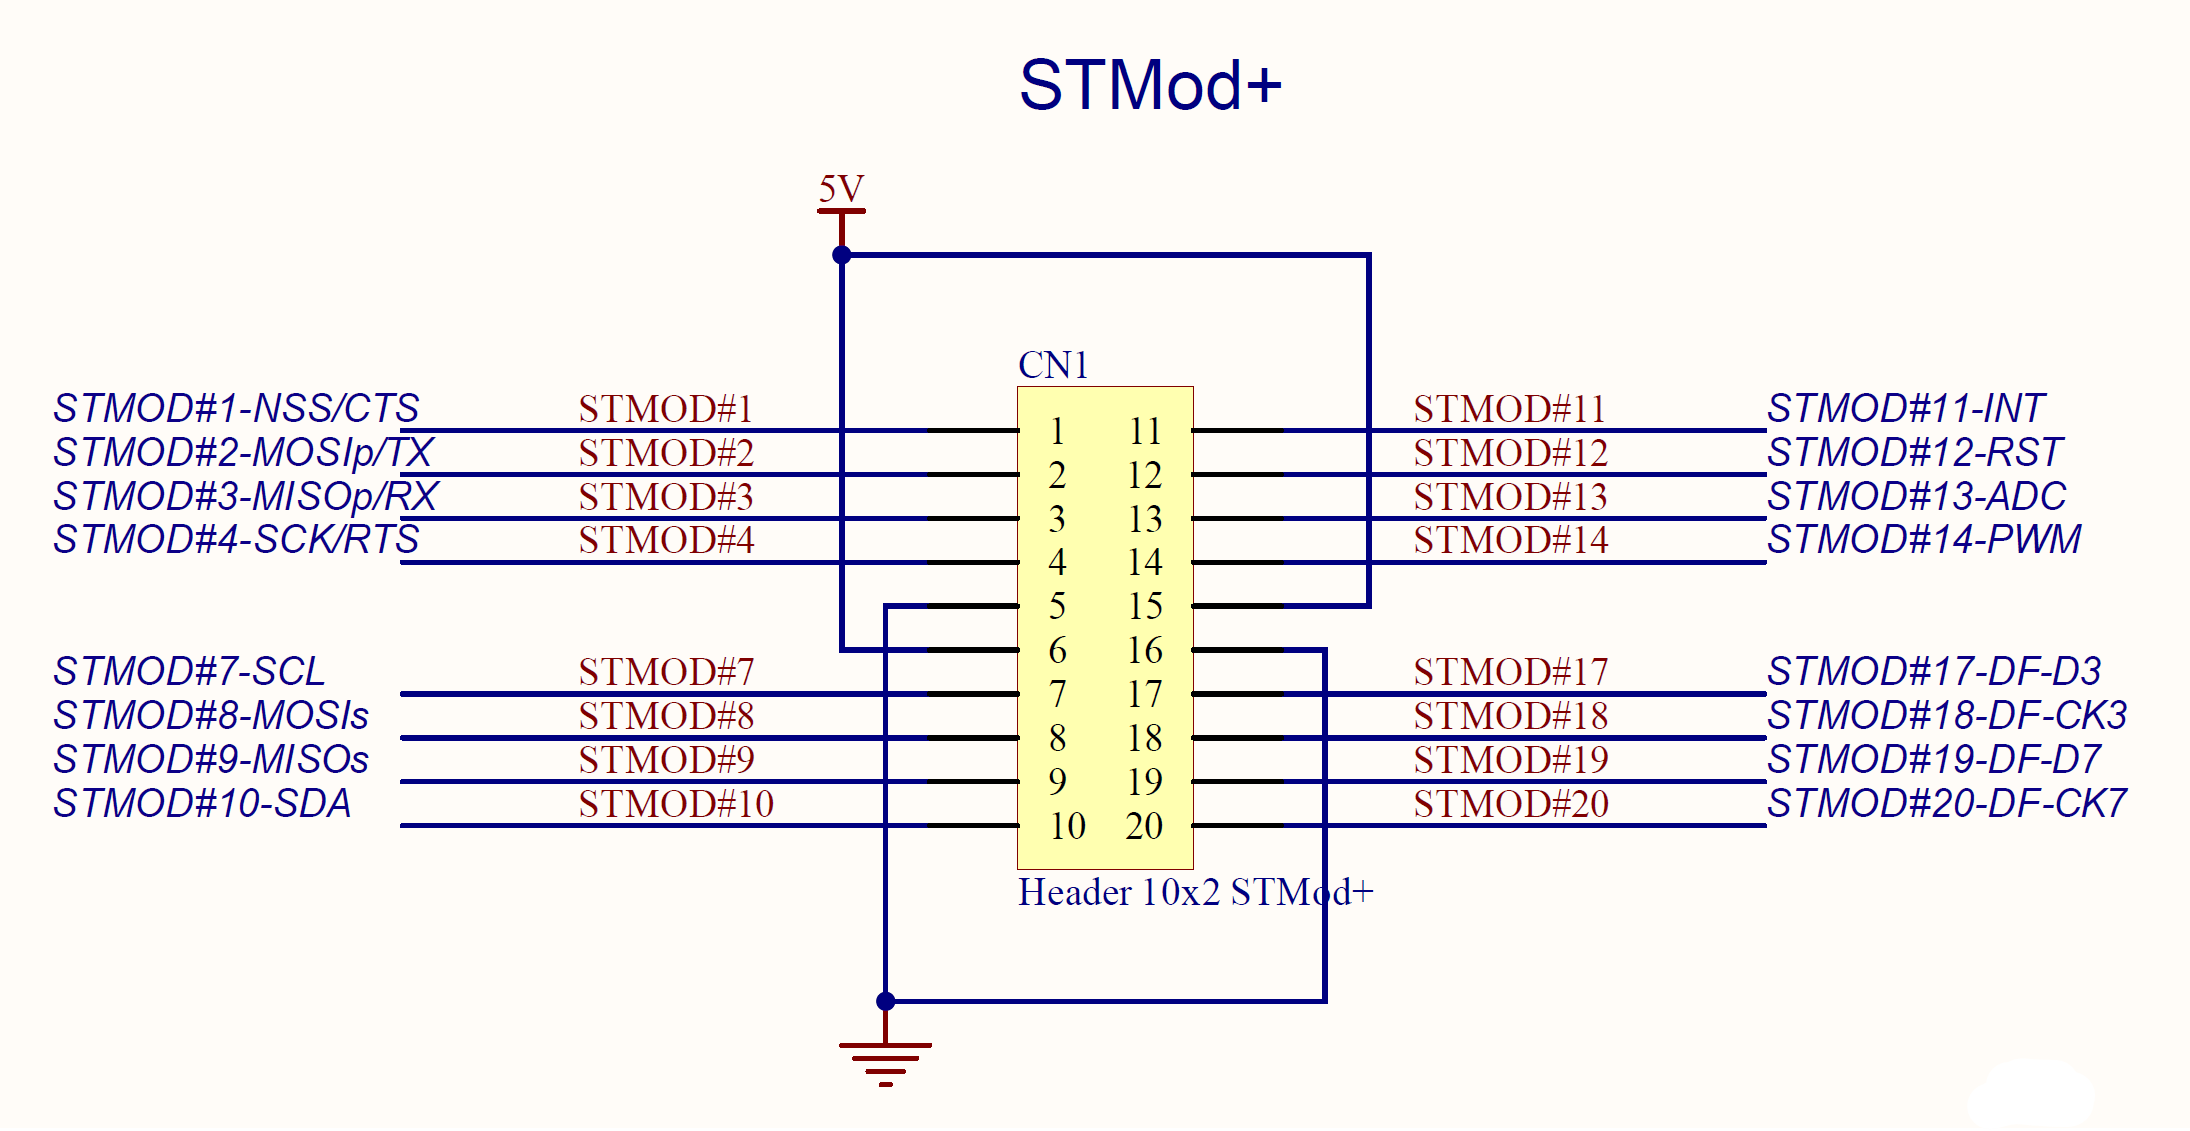
\includegraphics[width=13cm]{Resources/Pictures/STMOD_Interface.png}
	\caption{STMod+ Interface}
	\label{fig:STMod+ Interface}
\end{figure}




\newpage

\subsection{Hardware concept}

After some thoughts I came up with the following HW concept.


\begin{figure}[H]
	\centering



    \tikzstyle{block} = [draw, fill=white, rectangle, 
    minimum height=3em, minimum width=6em]
    \tikzstyle{sum} = [draw, fill=white, circle, node distance=1cm]
    \tikzstyle{input} = [coordinate]
    \tikzstyle{output} = [coordinate]
    \tikzstyle{pinstyle} = [pin edge={to-,thin,black}]

    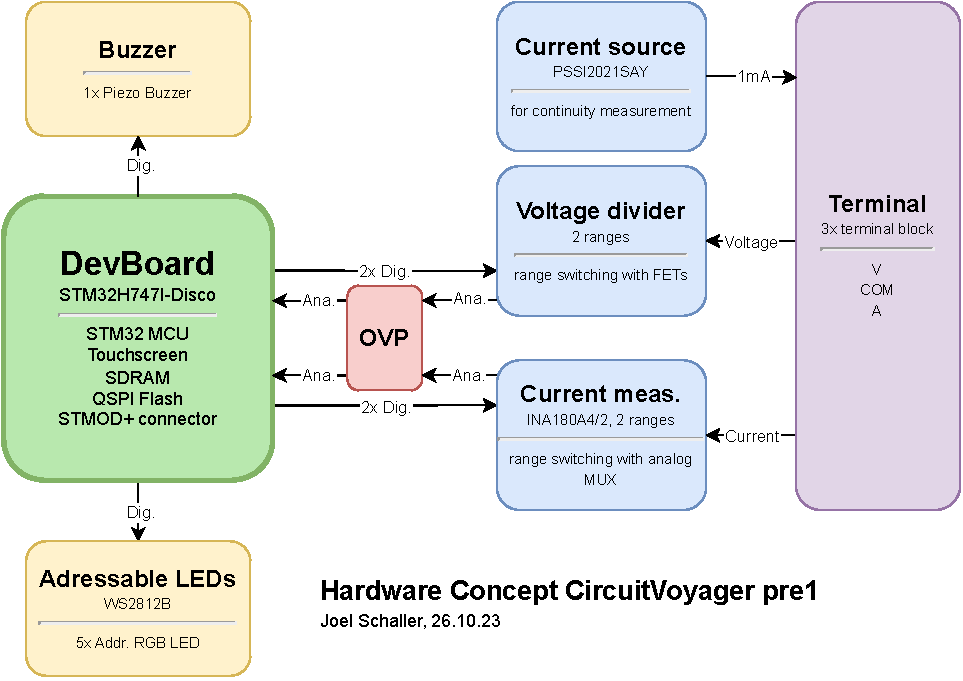
\includegraphics[width=15cm]{Resources/Pictures/Hardware_Concept_CircuitVoyager_pre1.pdf}

    \vspace{0.2cm}

	\caption{Extension PCB HW concept}
	\label{fig:Extension PCB HW concept}
\end{figure}

\subsubsection{Voltage measurement}
To measure voltage, the DUT should be connected to the terminals V and COM. COM is connected internally to device GND. The V terminal is connected to the Voltage divider block. This block divides the input voltage down, so the ADC in the MCU doesn't overshoot. There are 2 ranges to measure voltage, which can be chosen by setting 2 digital output, that go from the MCU to the voltage divider. There's also an OVP, to protect the MCU from voltages higher than 3.3V. \cite{DMM_Video_ElectroNoobs}

\subsubsection{Current measurement}
To measure current, the DUT should be connected to the terminals A and COM. COM is connected internally to device GND. The A terminal is connected to current measurement block. This block measures the current, by letting the current flow through one of two shunt resistors. The DMM can choose which resistor and therefore range should be selected with the 2 digital Output that are connected from the MCU to the current measurement block. The voltage over the selected shunt is then amplified, by a current amplifier IC and then measured by the MCUs ADC. There's also an OVP, to protect the MCU from voltages higher than 3.3V. \cite{DMM_Video_ElectroNoobs}

\subsubsection{Continuity measurement}
To measure continuity, both the voltage divider and the current source is used. The continuity between the V and COM pins is measured. For this a constant current produced by the current source is flowing out of the V terminal. Simultaneously the voltage across those terminals is measured and the resistance / continuity can be evaluated. If continuity is detected, either the buzzer beeps or the LEDs blink. \cite{DMM_Video_ElectroNoobs}



\subsection{Schematic}
The schematic took me a bit longer than usual, because it's my first whole HW project in Altium before I used KiCAD and Altium is a lot more features and in my opinion is harder to learn. The schematic is in the Appendix [CHAPTER!!!! :)].

\subsubsection{Buzzer Circuit}

\begin{figure}[H]
	\centering
	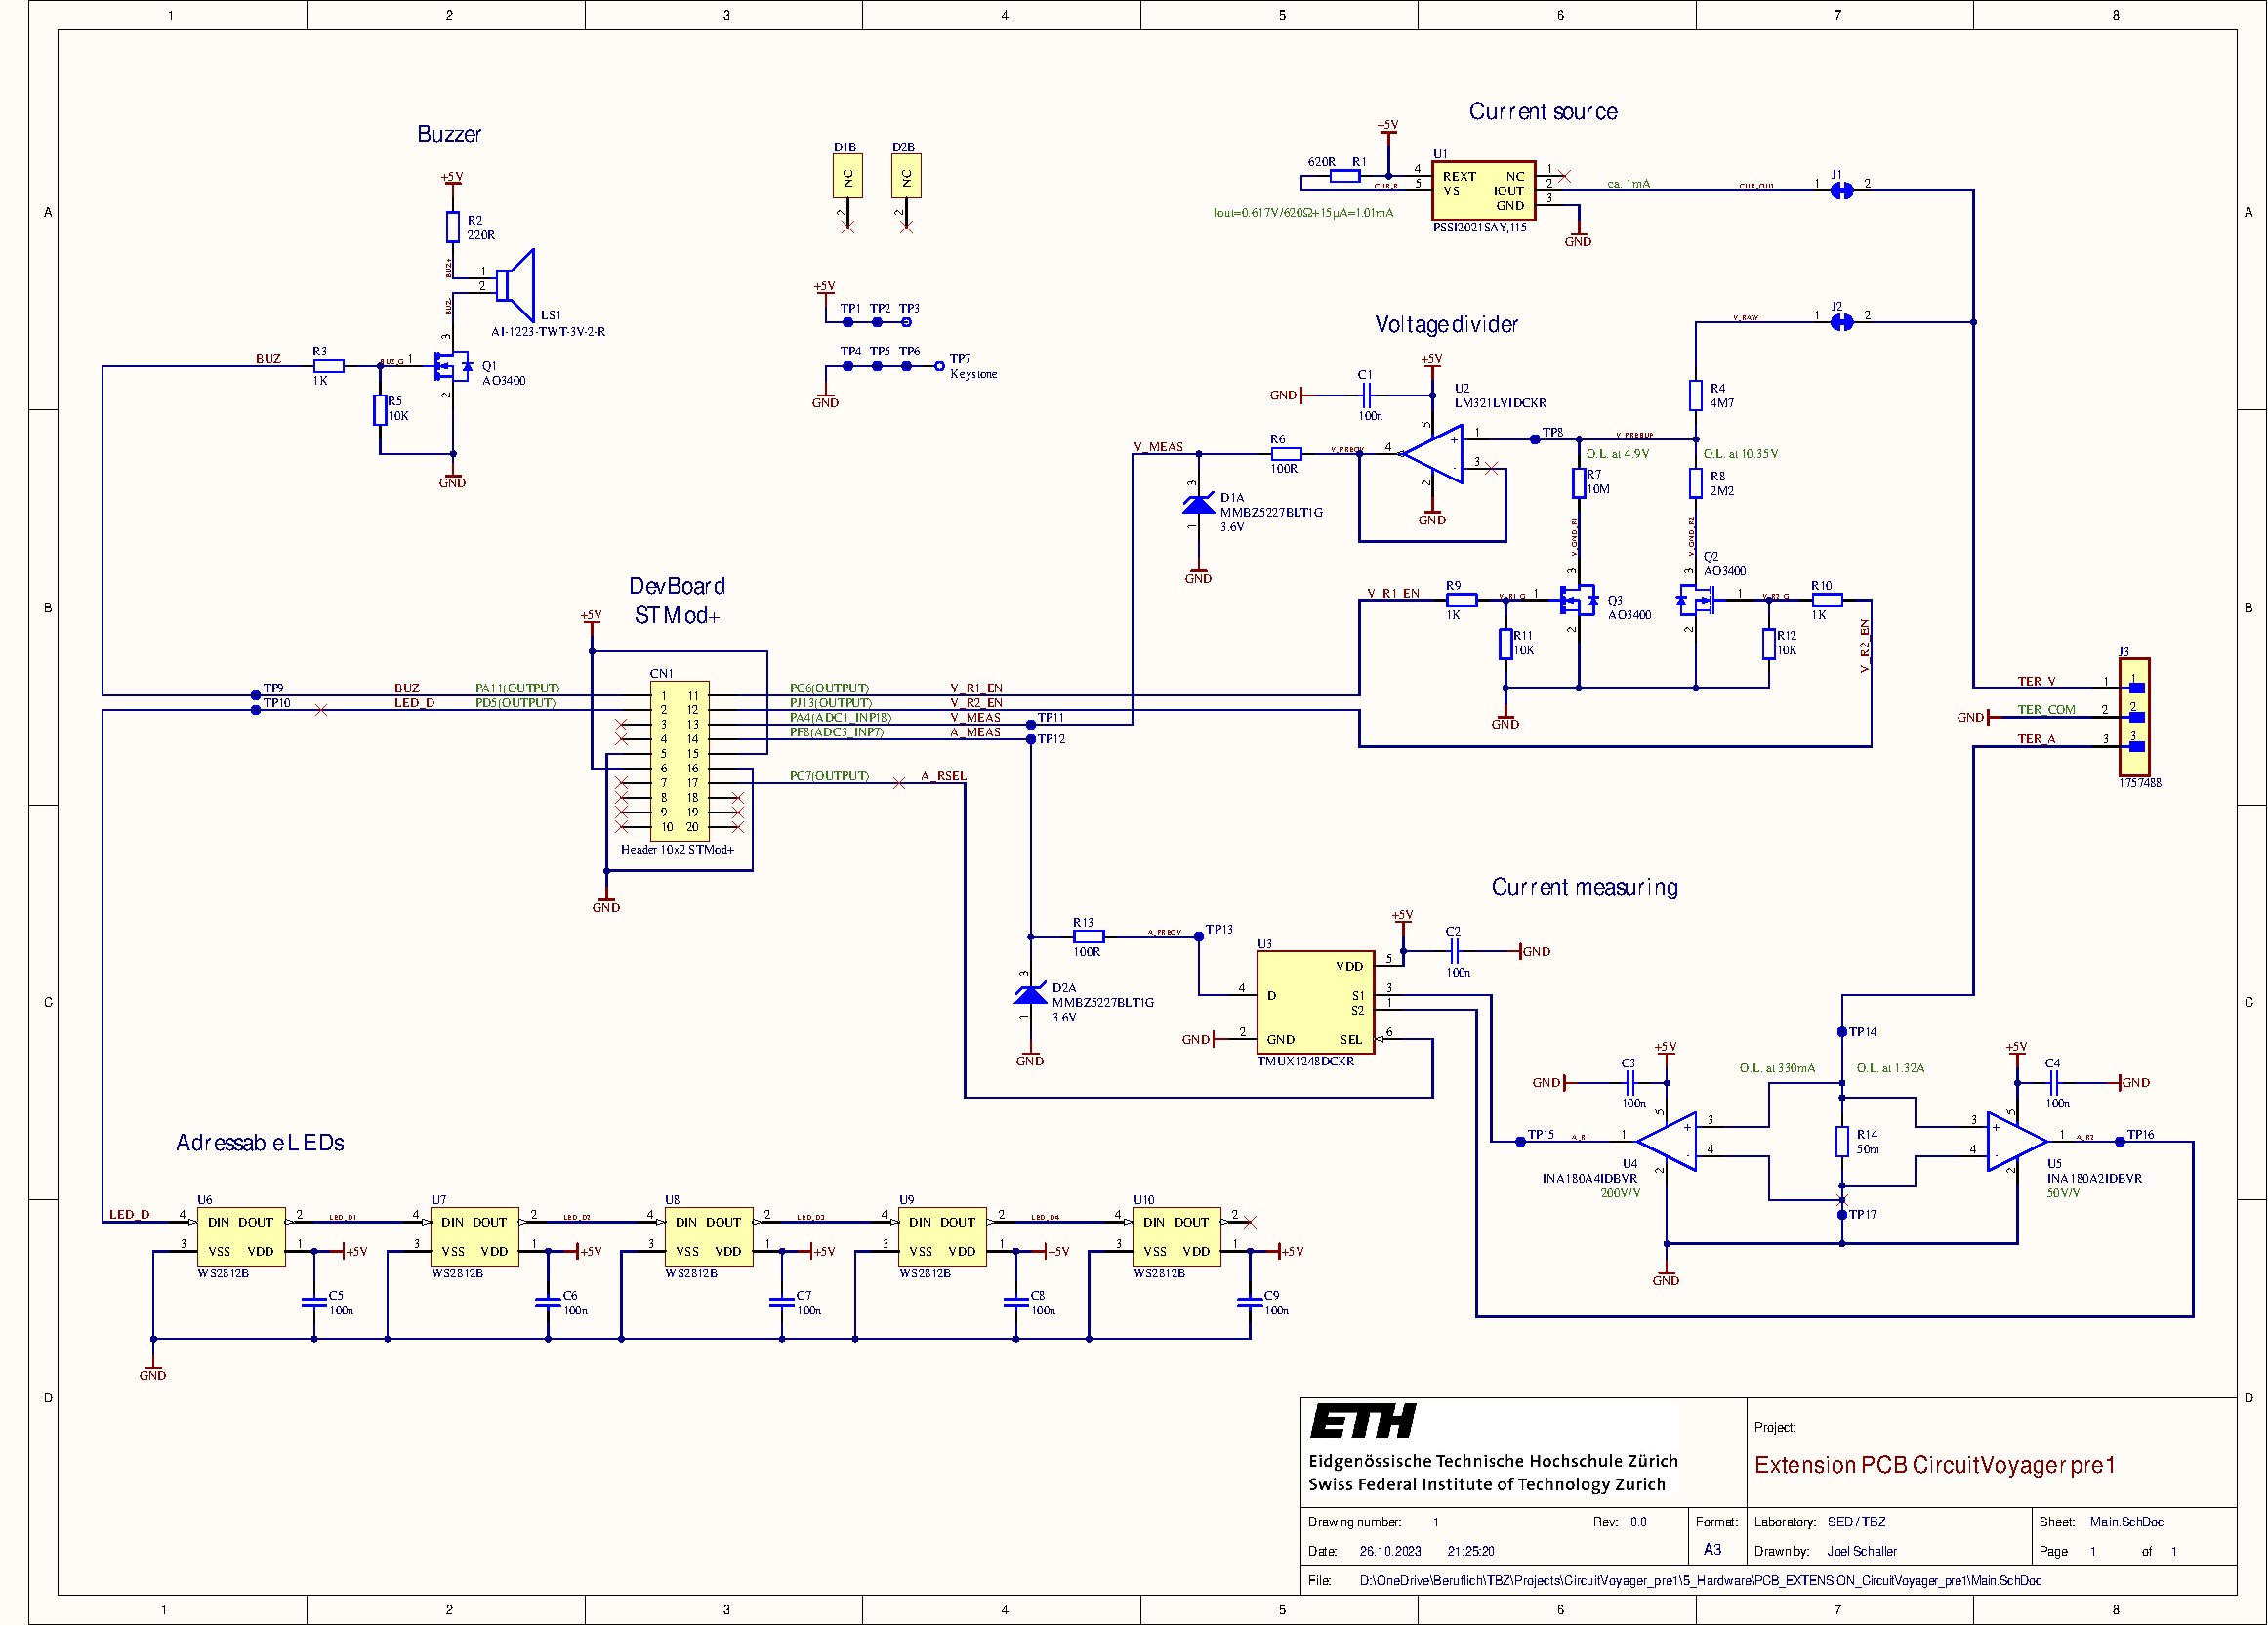
\includegraphics[width=8cm, trim={3.4cm 19cm 28.5cm 2cm}, clip]{Resources/Pictures/Schematic_PCB_EXTENSION_CircuitVoyager_pre1.pdf}
	\caption{Buzzer Circuit}
	\label{fig:Buzzer Circuit}
\end{figure}

This is an active buzzer. If the BUZ line is pulled high by the MCU, the MOSFET starts to conduct and the buzzer starts beeping. This circuit will be used to give an acoustic feedback to the user, if for example a continuity has been detected. 

The resistors R3 and R5 build a voltage divider with a ratio of 1/10. This has the advantage, that the gate capacitance of Q1 is charged with a limited current and if nothing's connected to the BUZ net the MOSFET turns the buzzer off and the whole machine isn't  in an indeterminate state.

The resistor R2 limit the current flowing through LS1. As LS1 is rated for 30mA at 3V.

\[R_2=\frac{U_{VCC}-U_{LS1}}{I_{LS1}}=\frac{5V-3V}{30mA}=66.\overline{6}\Omega\]
\[P_{R2}=I^2 \cdot R=(30mA)^2 \cdot 66. \overline{6} \Omega =60mW\]

Finally, I've chosen a 220\(\Omega\) resistor for R2. With this value the sound should be enough loud, that the user hears it. And the power loss of the resistor will be smaller. That means it should be perfectly fine to use a 0402 resistor that is rated for 62.5mW.


\subsubsection{Adressable LEDs Circuit}

\begin{figure}[H]
	\centering
	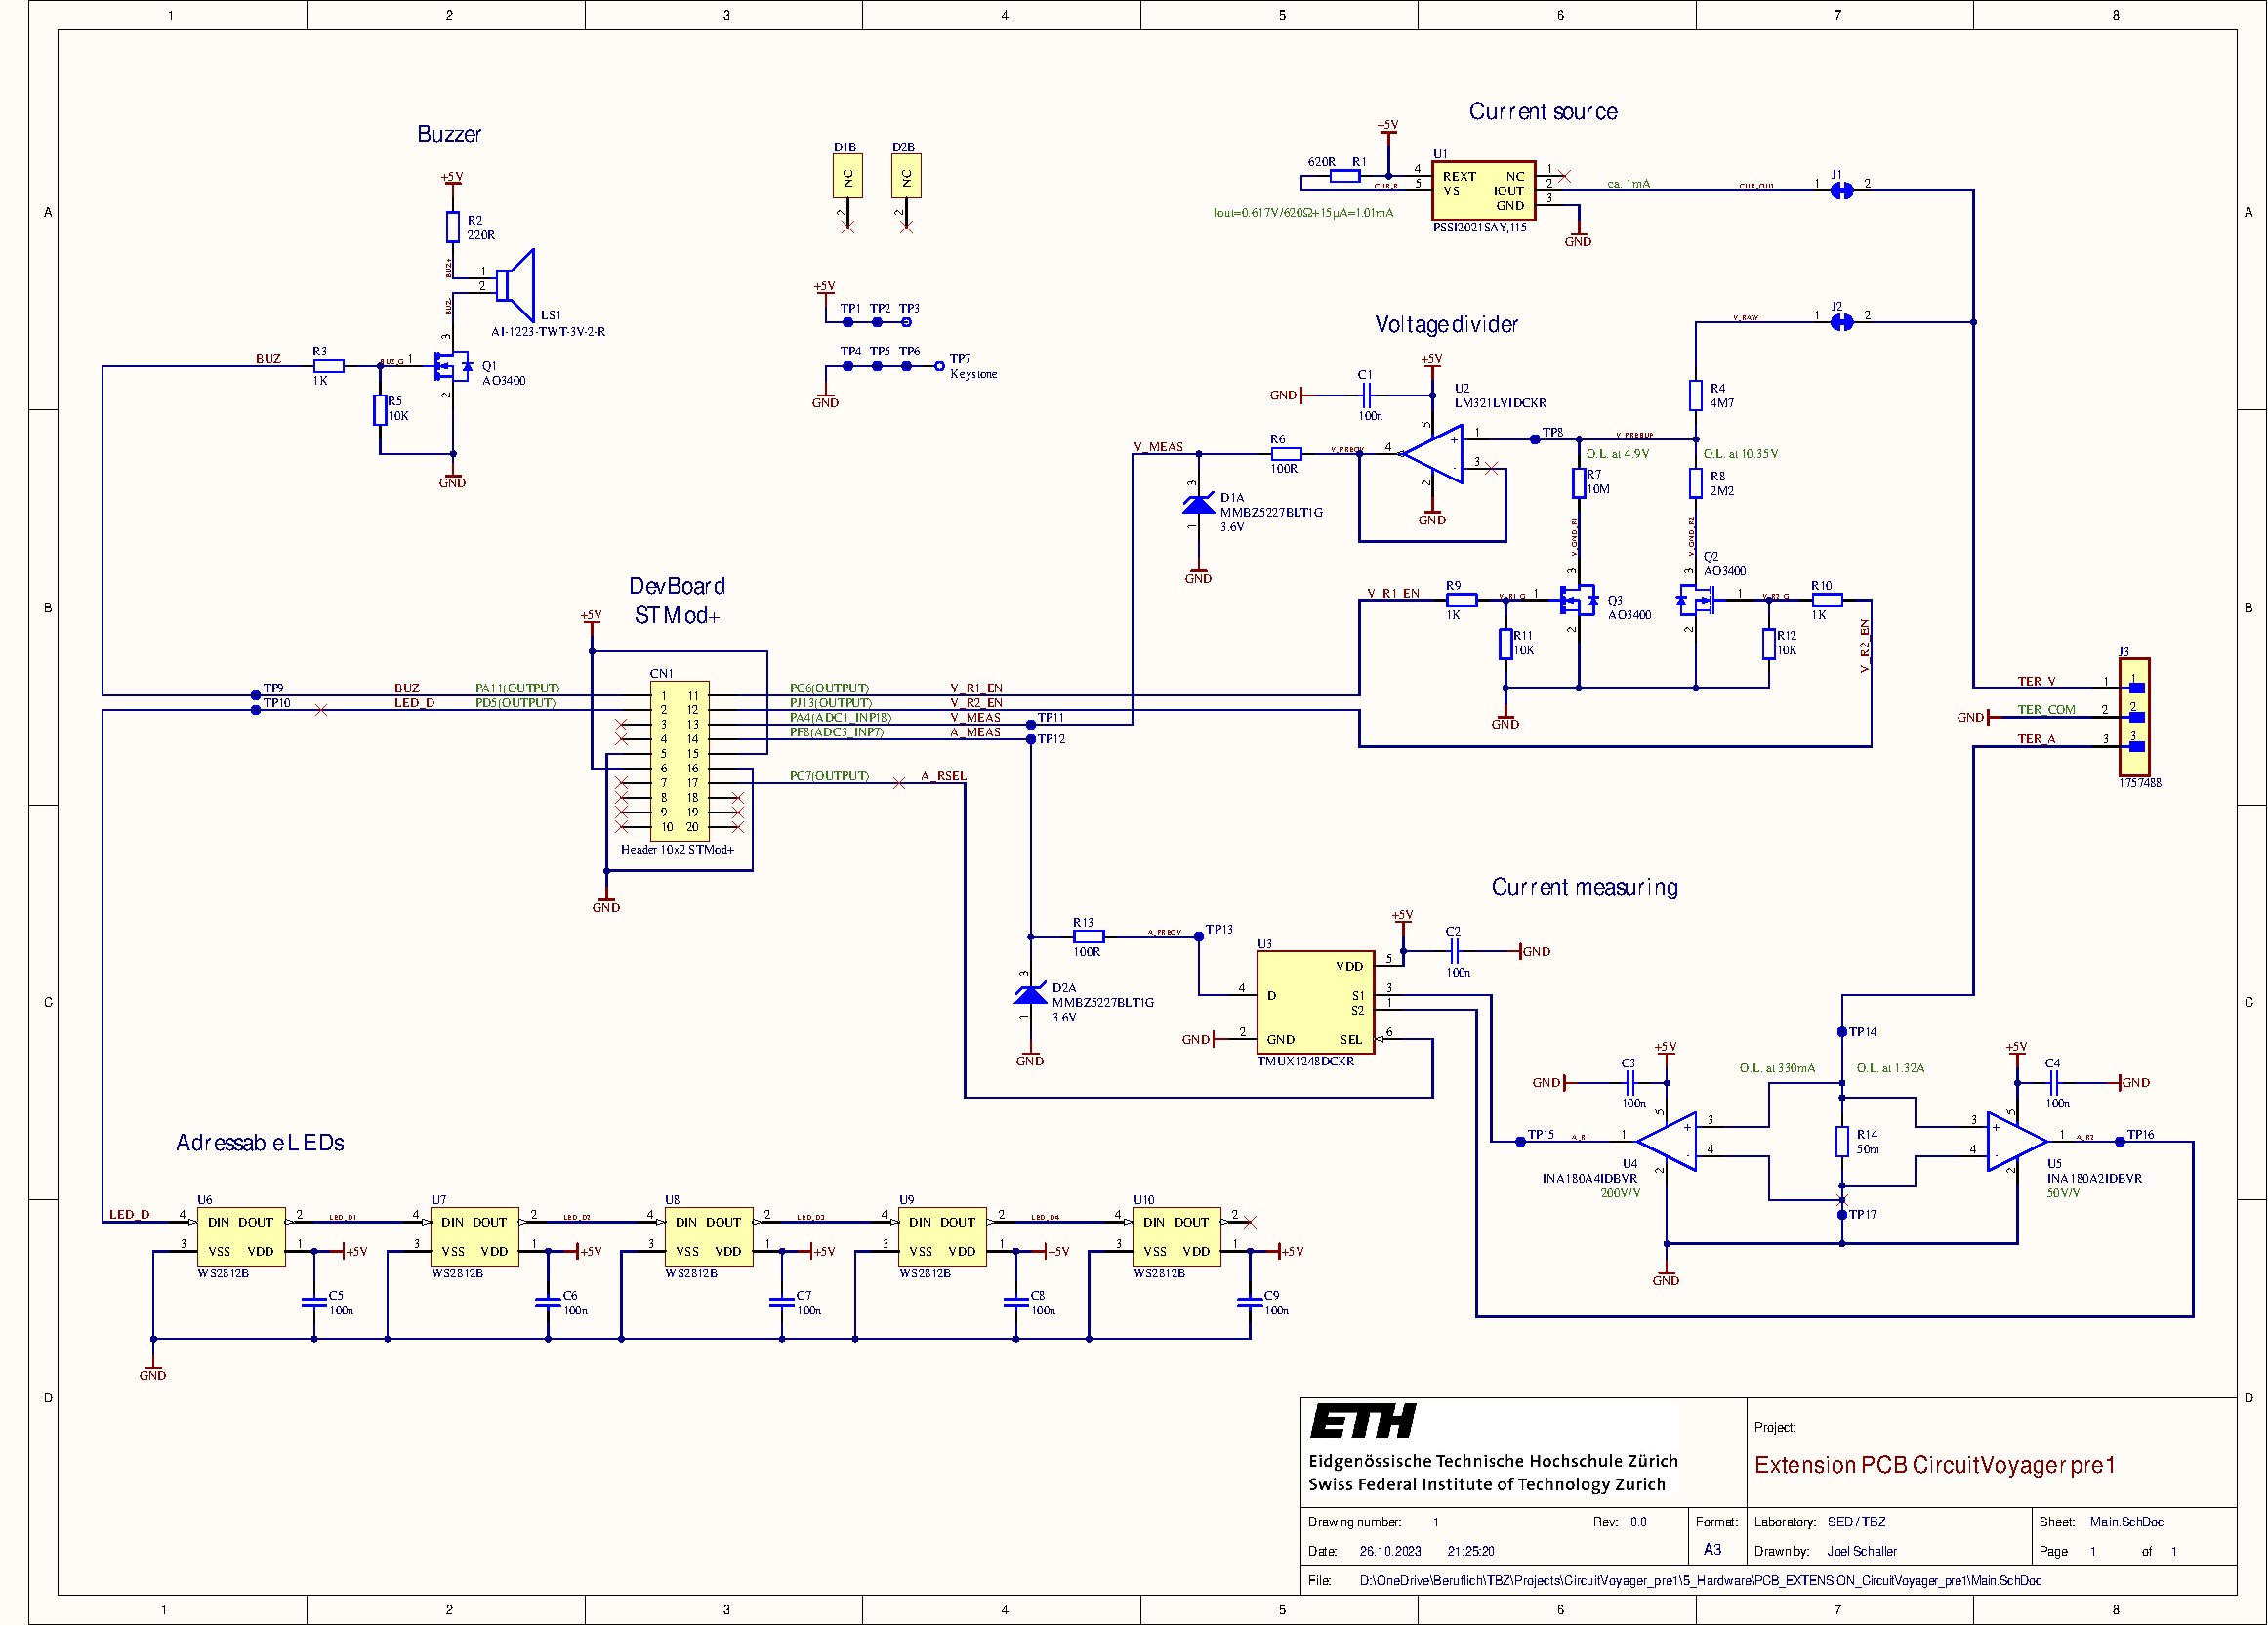
\includegraphics[width=15cm, trim={1.3cm 4cm 16.3cm 20cm}, clip]{Resources/Pictures/Schematic_PCB_EXTENSION_CircuitVoyager_pre1.pdf}
	\caption{Adressable LEDs Circuit}
	\label{fig:Adressable LEDs Circuit}
\end{figure}

An other option to show if continuity has been detected are these LEDs. The advantage of them is, that they only need one data connection and already include their logic and driving circuits. I've equiped the with one bulk C each, because they're integrated components and they're driven over the 5V rail, which they're specified for. But if they're driven by 5V they theoretically detect all voltages over 3.5V as a logical high. But the MCU only output 3.3V. I've used those LEDs much in past projects and this was never a problem, so I'm assuming that it should also work this time.
